\section{Architecture}
\index{WebRTC}{WebRTC} uses different networking techniques to create a connection between peers. We will explore those techniques and technologies in this chapter.

\subsection{Network Address Translation (\index{NAT}{NAT})}
Devices in a network need a public IP address assigned so traffic from outside the network can be routed to the correct destination, this is done by using \index{NAT}{NAT}. The router will translate requests from a source's private \index{IP}{IP} to to the routers public \index{IP}{IP} with a unique \index{port}{port}. The goal is to not need a unique public \index{IP}{IP} for each device.

\clearpage
\subsection{Session Traversal Utilities for \index{NAT}{NAT} (\index{STUN}{STUN})}
\index{STUN}{STUN} is used to find the public \index{IP}{IP} of a peer to which will be connected later on. It also can determine if there are any network restrictions in place which would prevent a connection, such as '\index{Symmetric NAT}{Symmetric NAT}'.

The peer sends a 'who am i' request to a \index{STUN}{STUN} server which responds with the public address of the peer.

\begin{figure}[H]
	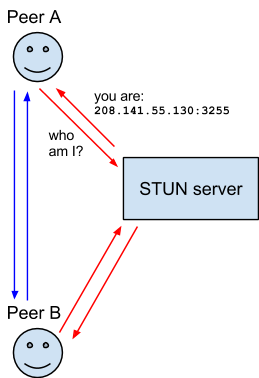
\includegraphics[scale=0.5]{images/webrtc-stun.png}
	\centering
	\caption{\index{STUN}{STUN} communication schema, \url{https://developer.mozilla.org/en-US/docs/Web/API/WebRTC_API/Protocols}}
	\label{fig:STUN}
\end{figure}

Here are some public available example \index{STUN}{STUN} servers:
\begin{itemize}
	\item stun.l.google.com:19302
	\item stun[1-4].l.google.com:19302
	\item stunserver.org
	\item stun.schlund.de
	\item stun.voipstunt.com
\end{itemize}

\clearpage
\subsection{Traversal Using Relays around \index{NAT}{NAT} (\index{TURN}{TURN})}
If \index{STUN}{STUN} can't be used, because for example '\index{Symmetric NAT}{Symmetric NAT}' is employed in the network, \index{TURN}{TURN} will be used as fallback. This is achieved by opening a connection with a \index{TURN}{TURN} server, this connection then will relaying all information through that server.

\begin{figure}[H]
	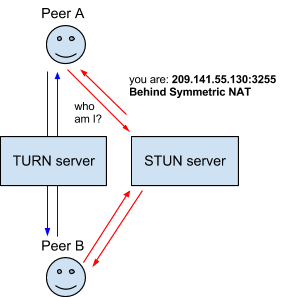
\includegraphics[scale=0.5]{images/webrtc-turn.png}
	\centering
	\caption{\index{TURN}{TURN} communication schema, \url{https://developer.mozilla.org/en-US/docs/Web/API/WebRTC_API/Protocols}}
	\label{fig:TURN}
\end{figure}

There are open \index{TURN}{TURN} servers available, for example provided by google. But this will mean all communication is going unprotected through a foreign server which might not be acceptable.

\subsection{Session Description Protocol (SDP)}
This standard describes the multimedia content of a connection. This includes a resolution, formats, codecs, encryption, etc. basically it is the metadata describing the content not the content itself.

\subsection{Interactive Connectivity Establishment (\index{ICE}{ICE}) Candidates}
Peers have to exchange information about the network connection, this is known as an \index{ICE}{ICE} candidate. Each peer proposes its best candidate, and will work down to the worst candidate until they agree on a common candidate.

\clearpage
\subsection{Complete Communication Schema}
The following figure gives an overview over the complete communication mechanism and its fallbacks.

\begin{figure}[H]
	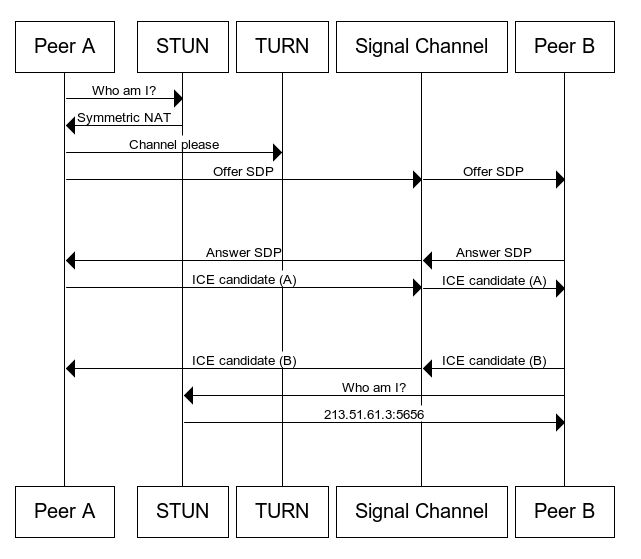
\includegraphics[scale=0.5]{images/webrtc-complete-diagram.png}
	\centering
	\caption{\index{WebRTC}{WebRTC} Complete communication schema, \url{https://developer.mozilla.org/en-US/docs/Web/API/WebRTC_API/Connectivity}}
	\label{fig:WebRTC}
\end{figure}
